% !TeX root = ../proceedings.tex

\section{Design Challenges}
\subsection{Accessibility}
To manoeuvre around in any application, a menu is needed. The menu is something every user has experience with and it is typically the first thing a user is faced with when accessing an application. This means that a menu must be short, concise and consist of certain classic elements, that a user would assume to see on a menu.\\ A user needs a way to close the application. On mobile phones nowadays this can be done with 'return' buttons on the phone, but many applications have a built in exit function.\\
The user also needs to have some sort of options menu and guidelines. Stacking LEGO seems simple and intuitive, but all the operations and possibilities is something that can confuse a potential user, especially in and AR application. \\
Lastly it shouldn't be complicated for the user to start a new LEGO session.
\subsection{A Main Menu}
To achieve accessibility a '5 plus 5' sketch generation session was held. Initially we thought about this application as a game, therefore the user would typically be met by a main menu screen, as figure \ref{fig:menu8} depicts.
\begin{figure}[t]
	\centering
	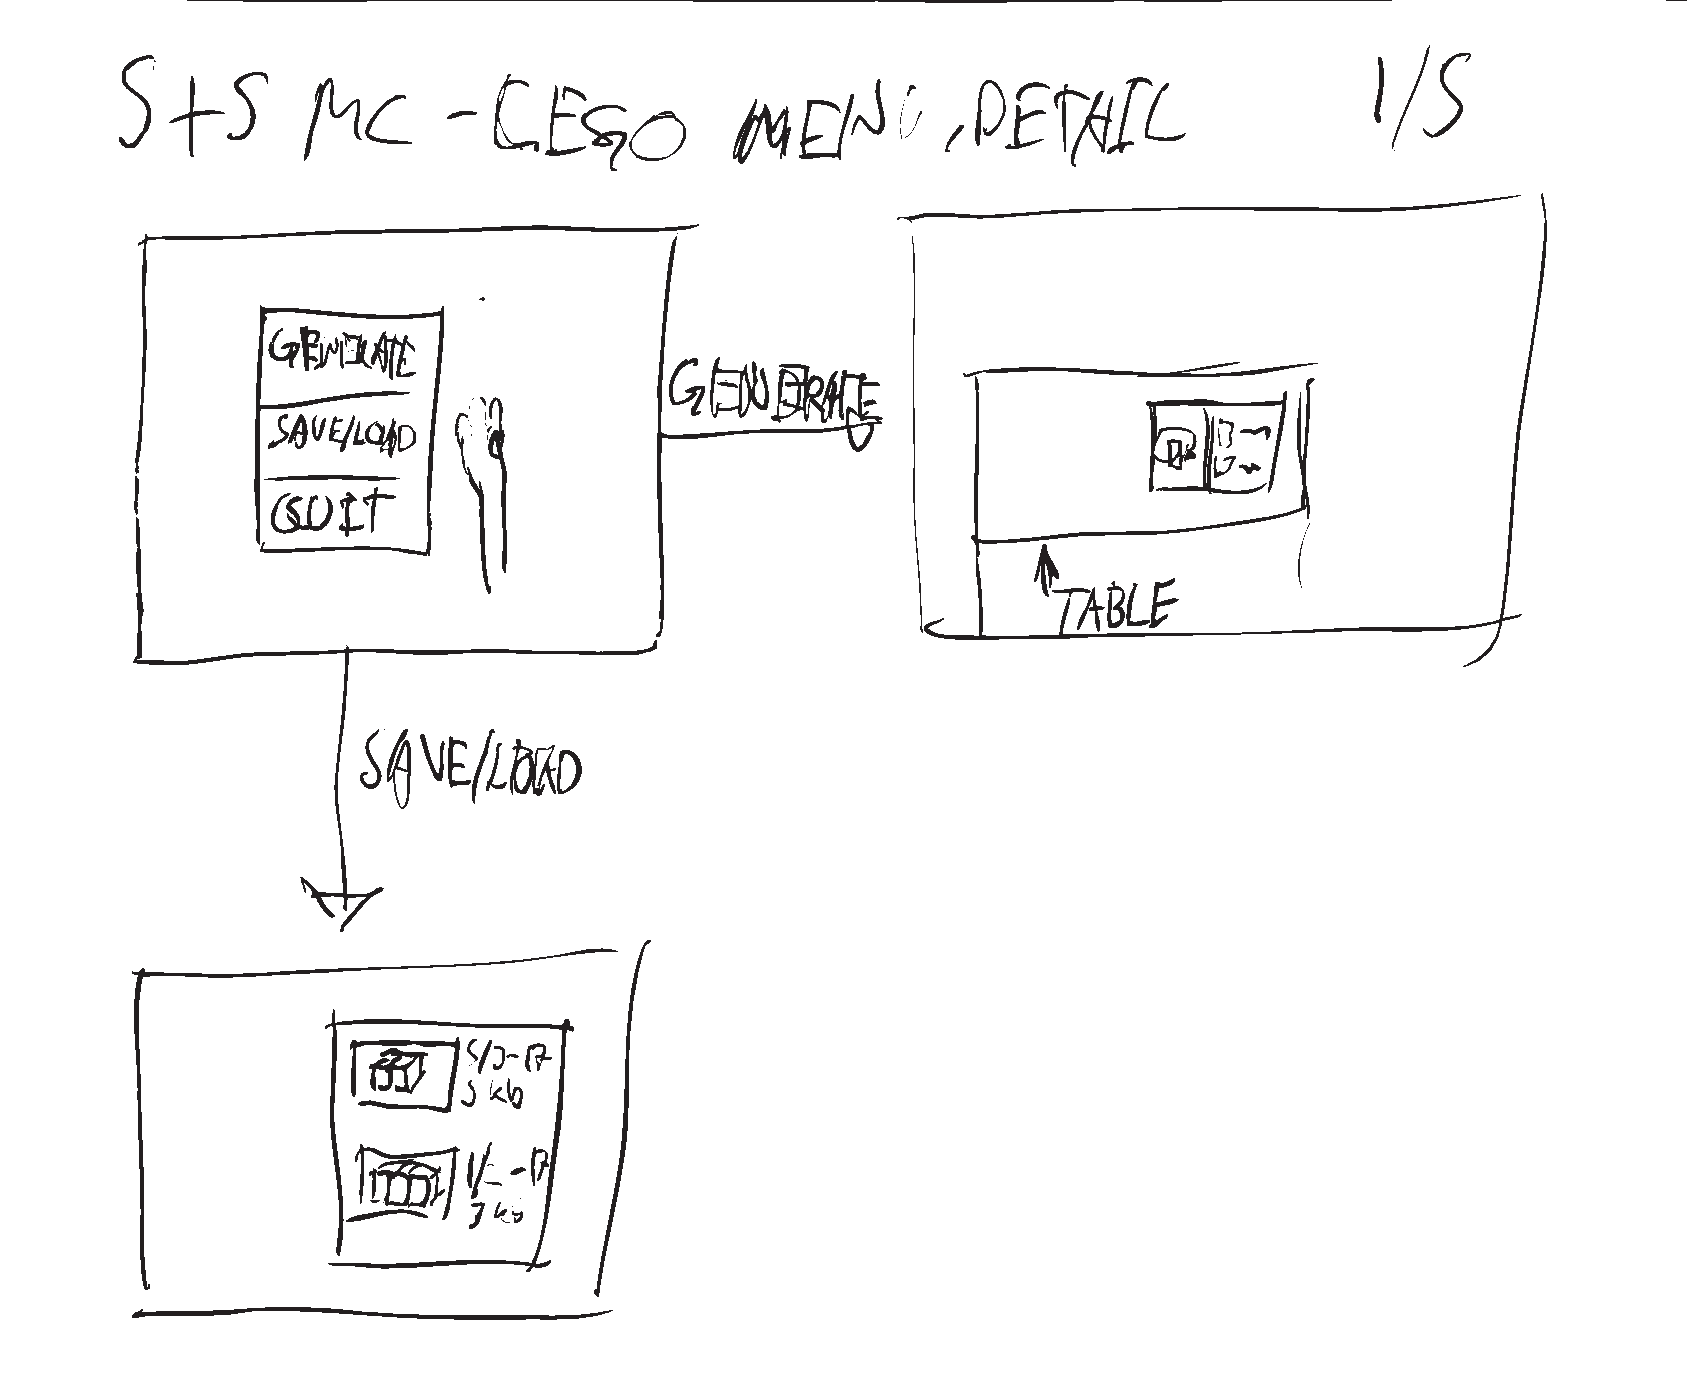
\includegraphics[width=210px]{figures/Menu/menu8_1.pdf}
	\caption{Initial sketch of a separate Main Menu}
	\label{fig:menu8}
\end{figure}
The initial idea was that the user would open the Hololens application, and be met with a menu screen, where actions such as generating a play area, loading/saving a game and a way to quit the application were possible. \\
One common theme in the sketching of the main menu was separating the design of the menu and the interaction techniques with the menu. The fact that we were working with the Hololens, led to some sketches being focused on the interaction, such as figure \ref{fig:menugesture} depicts,  while other sketches solely focused on the design of the menu.\\
\begin{figure}[t]
	\centering
	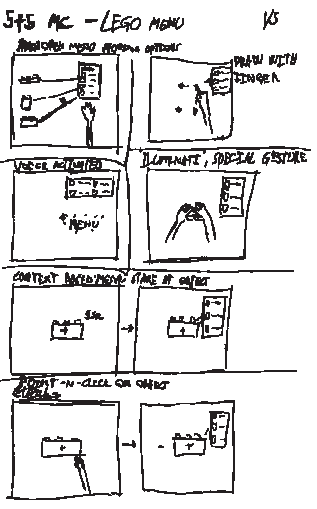
\includegraphics[width=210px]{figures/Menu/menu5_1.pdf}
	\caption{A focus on gestures rather than design, impacted the design. The figure shows different ways of creating an interactive menu with gestures.}
	\label{fig:menugesture}
\end{figure}
\\
The possibilities with the HoloLens gestures and the augmented reality made it apparent that the menu had to be moveable, either by closing and opening it at a new spot using the available gestures, or the ability to move it around and place it in favorable self-chosen spots.
\subsection{The Generator}
After discussing menus in the context of the Hololens, it became apparent that there was a need for a secondary menu that could be placed and interacted with while using the LEGO application. This menu should only interfere with the play area, and have functions tied to the bricks. Figure \ref{fig:genboard1} is a sketch of the functionalities the "Generator" could have, such as brick types and templates.
\begin{figure}[t]
	\centering
	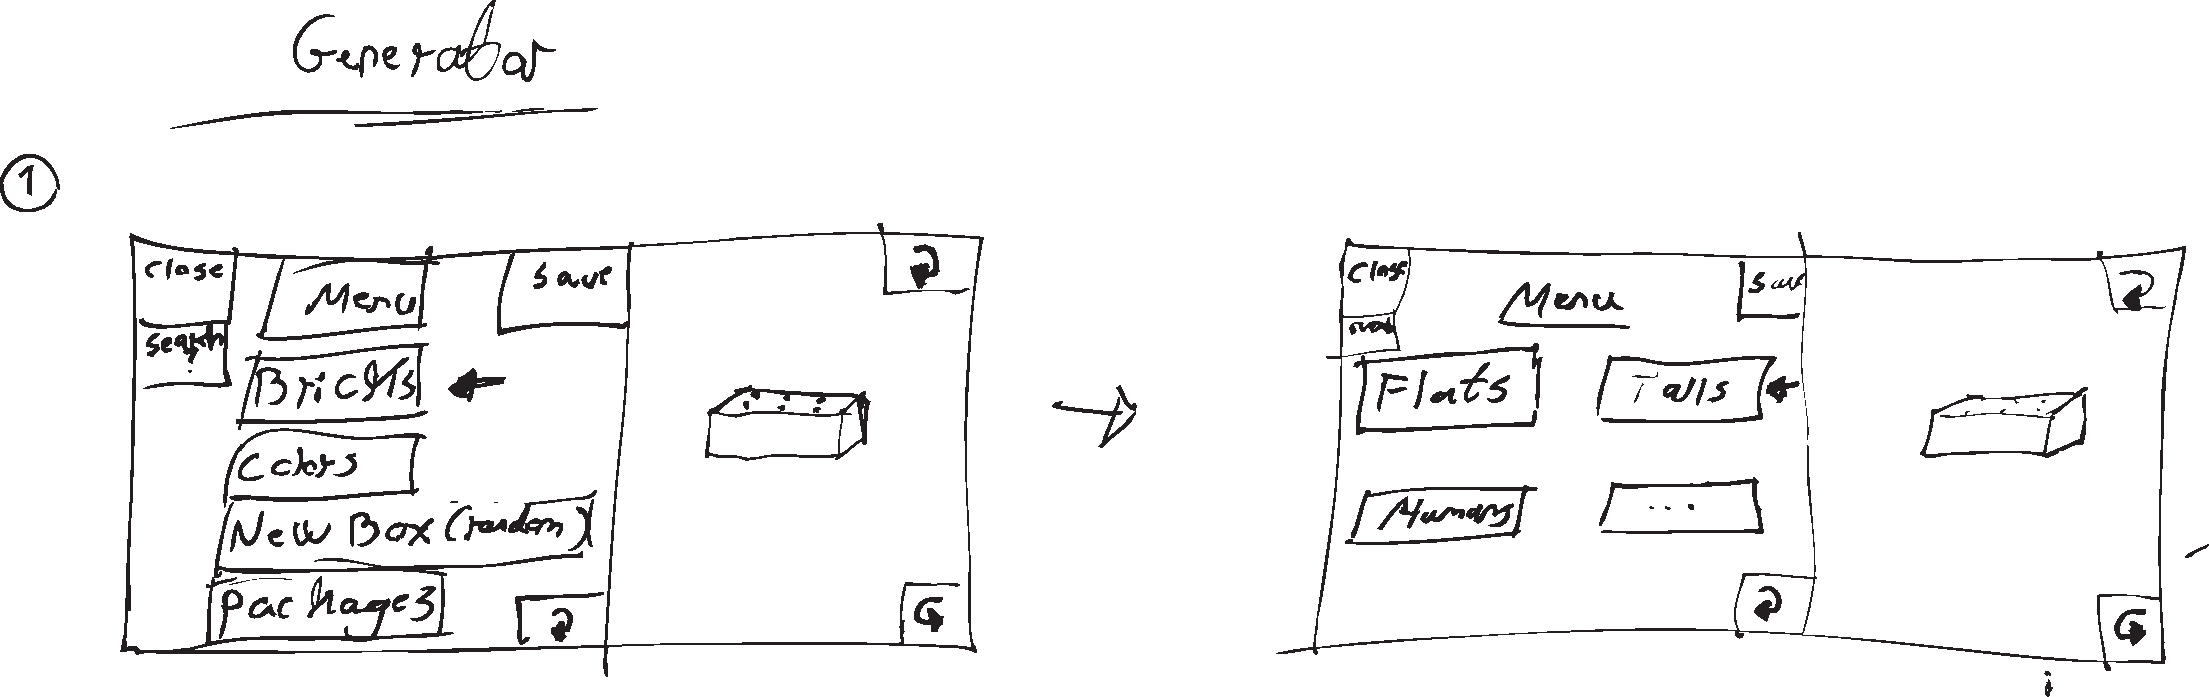
\includegraphics[width=210px]{figures/Generator/gen5_1.pdf}
	\caption{An initial sketch of how the generator could look like. The menu screen has alot of functionalities, and the actions chosen happen on the right side.}~\label{fig:genboard1}
\end{figure}
The generator should have functionalites that can alter the blocks, but it also needs to be interactive and moveable in the specified play area.\\
As Figure \ref{fig:gentablet} suggests, the generator could be placed on a table and used for generating bricks from that spot.
\begin{figure}[t]
	\centering
	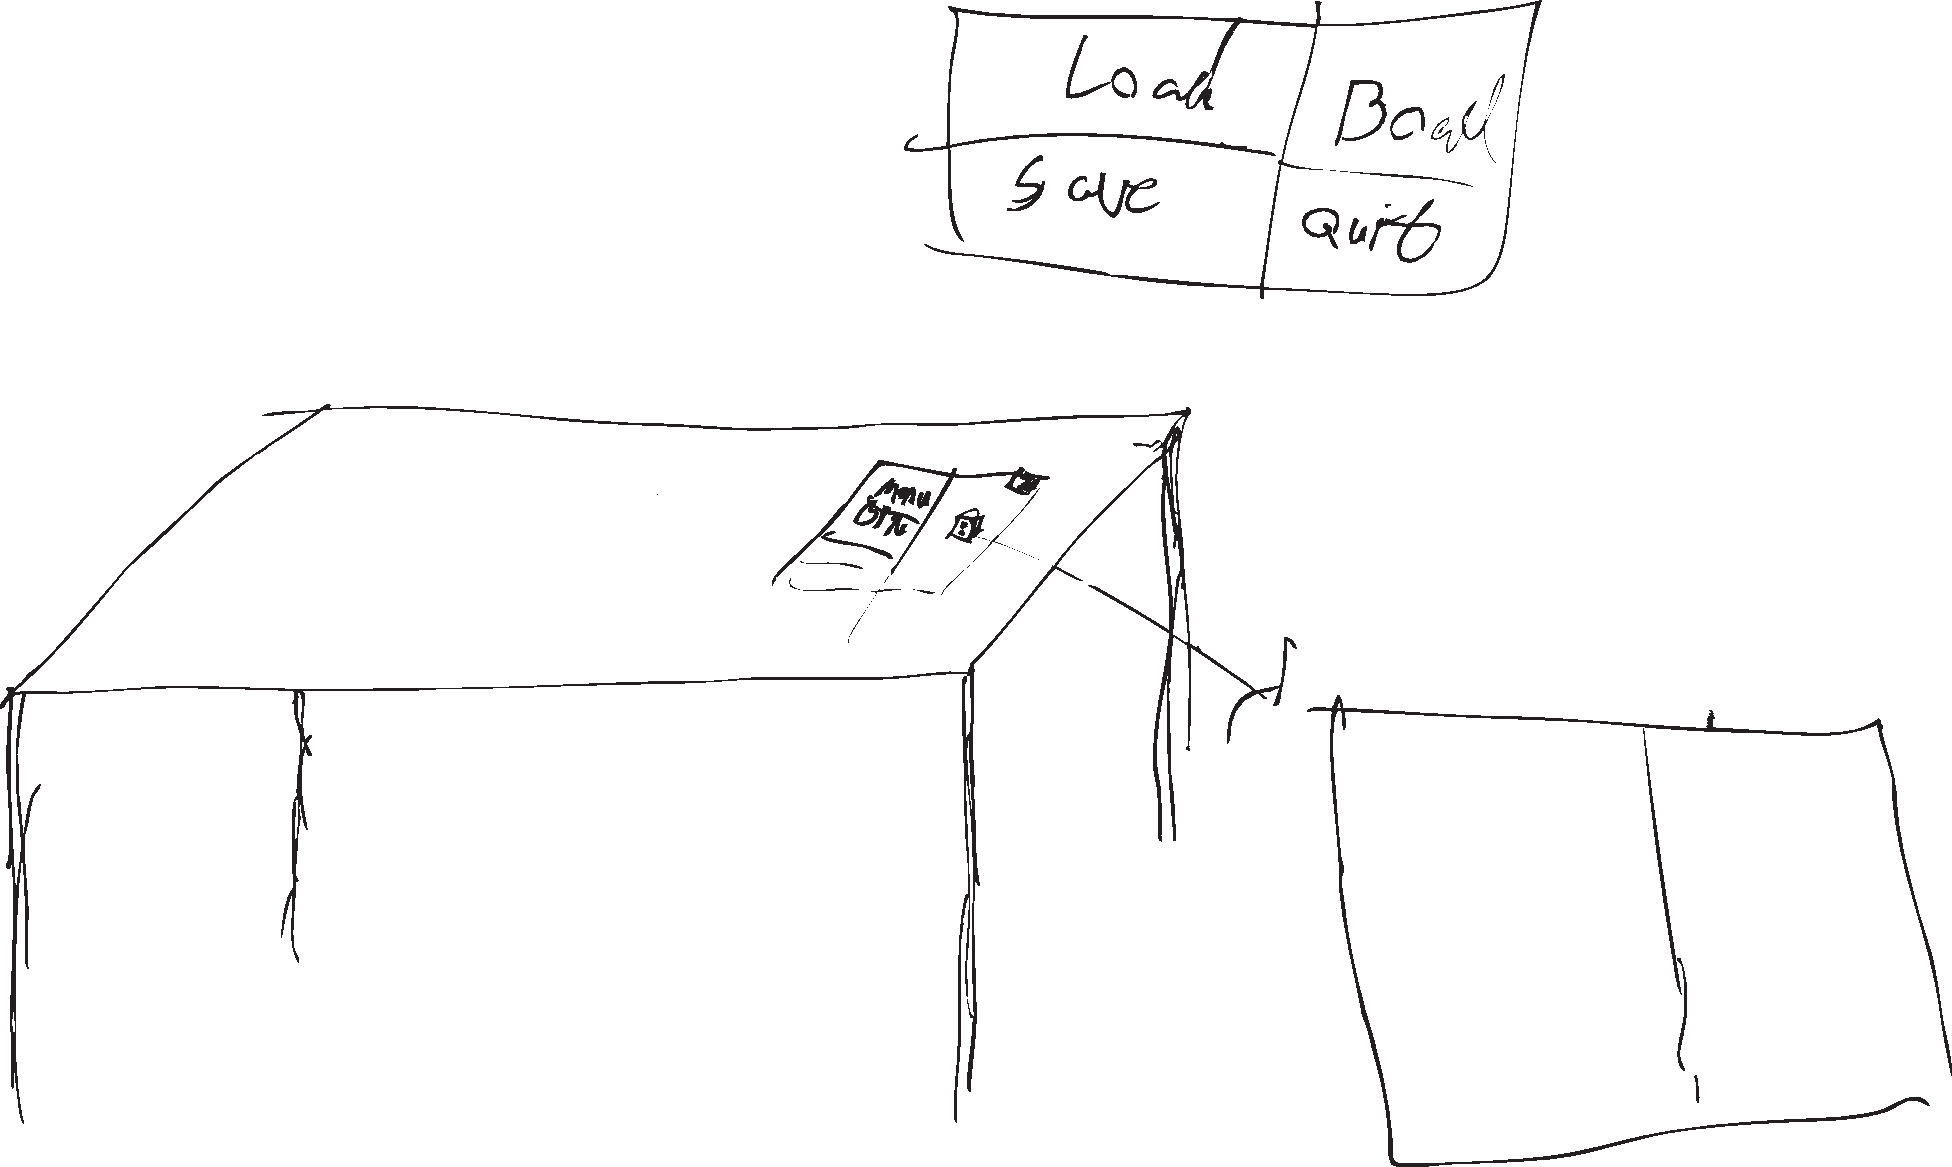
\includegraphics[width=210px]{figures/Generator/gen6_1.pdf}
	\caption{First sketch of the generator as a movable object. Here placed on the table, spawning blocks on the table.}~\label{fig:gentablet}
\end{figure}
We designed the generator as a virtual tablet device. Theory being that a tablet being a solid familar object, makes it more intuitive and natural for the user to interact with. To lift, move and place the tablet on a surface is hopefully a simple and familiar task for the user. To accompany the tablet device, a simple interface was designed. The interface only needed simple functions all tied to spawning and altering lego bricks. The user can spawn bricks of different types, change colors, save/load a play scene and spawn different prebuilt templates.
\subsection{Final Design}
During the sketching phase, several design choices were discussed. One of the very first concerns was the overall look of the main menu and the generator. The choice of big buttons, clear visual cues and short textual descriptions were present in almost all of the sketches in the early design phase. The need for a simple interface was a must, as stacking LEGO bricks shouldn't be a hassle. \\
We wanted an effective and efficient process of interacting with LEGO. We also wanted the users to experience the same satisfaction of building LEGO when using our application. Therefore the menus should not be overcomplicated in functions and design, but not sparse in functions either. To achieve these 3 key elements we designed the menu content with simple LEGO thumbnails, that explained what each button did along with simple textual descriptions. \\
As the development of the application progressed it became more  apparent that an actual main menu was not necessary. Using way too many menus in our simple interactive application would hinder the effectiveness and efficiency for the user, due to the limited functions our prototype had to offer. \\
To circumvent a clonky and cluttered experience for the user we decided on creating a tablet looking generator. Using a single solid object with all functionalities in the same place, would ease the user interaction. Instead of going through a main menu and then having the generator menu, which contains the functionality for working with the LEGO bricks, we decided on spawning the generator at the application start up. Due to the way our prototype works it seems as a natural choice to "cut out the middleman", here the main menu.  \\ 
Granted, with an eventual increase in functionality and complexity of the application, a root/main menu might prove useful as to not clutter the users experience when they are building as opposed to when they are in the main menu, where setting options, loading scenarios, downloading templates etc. would be a valid solution.\\
\begin{figure}[t]
	\centering
	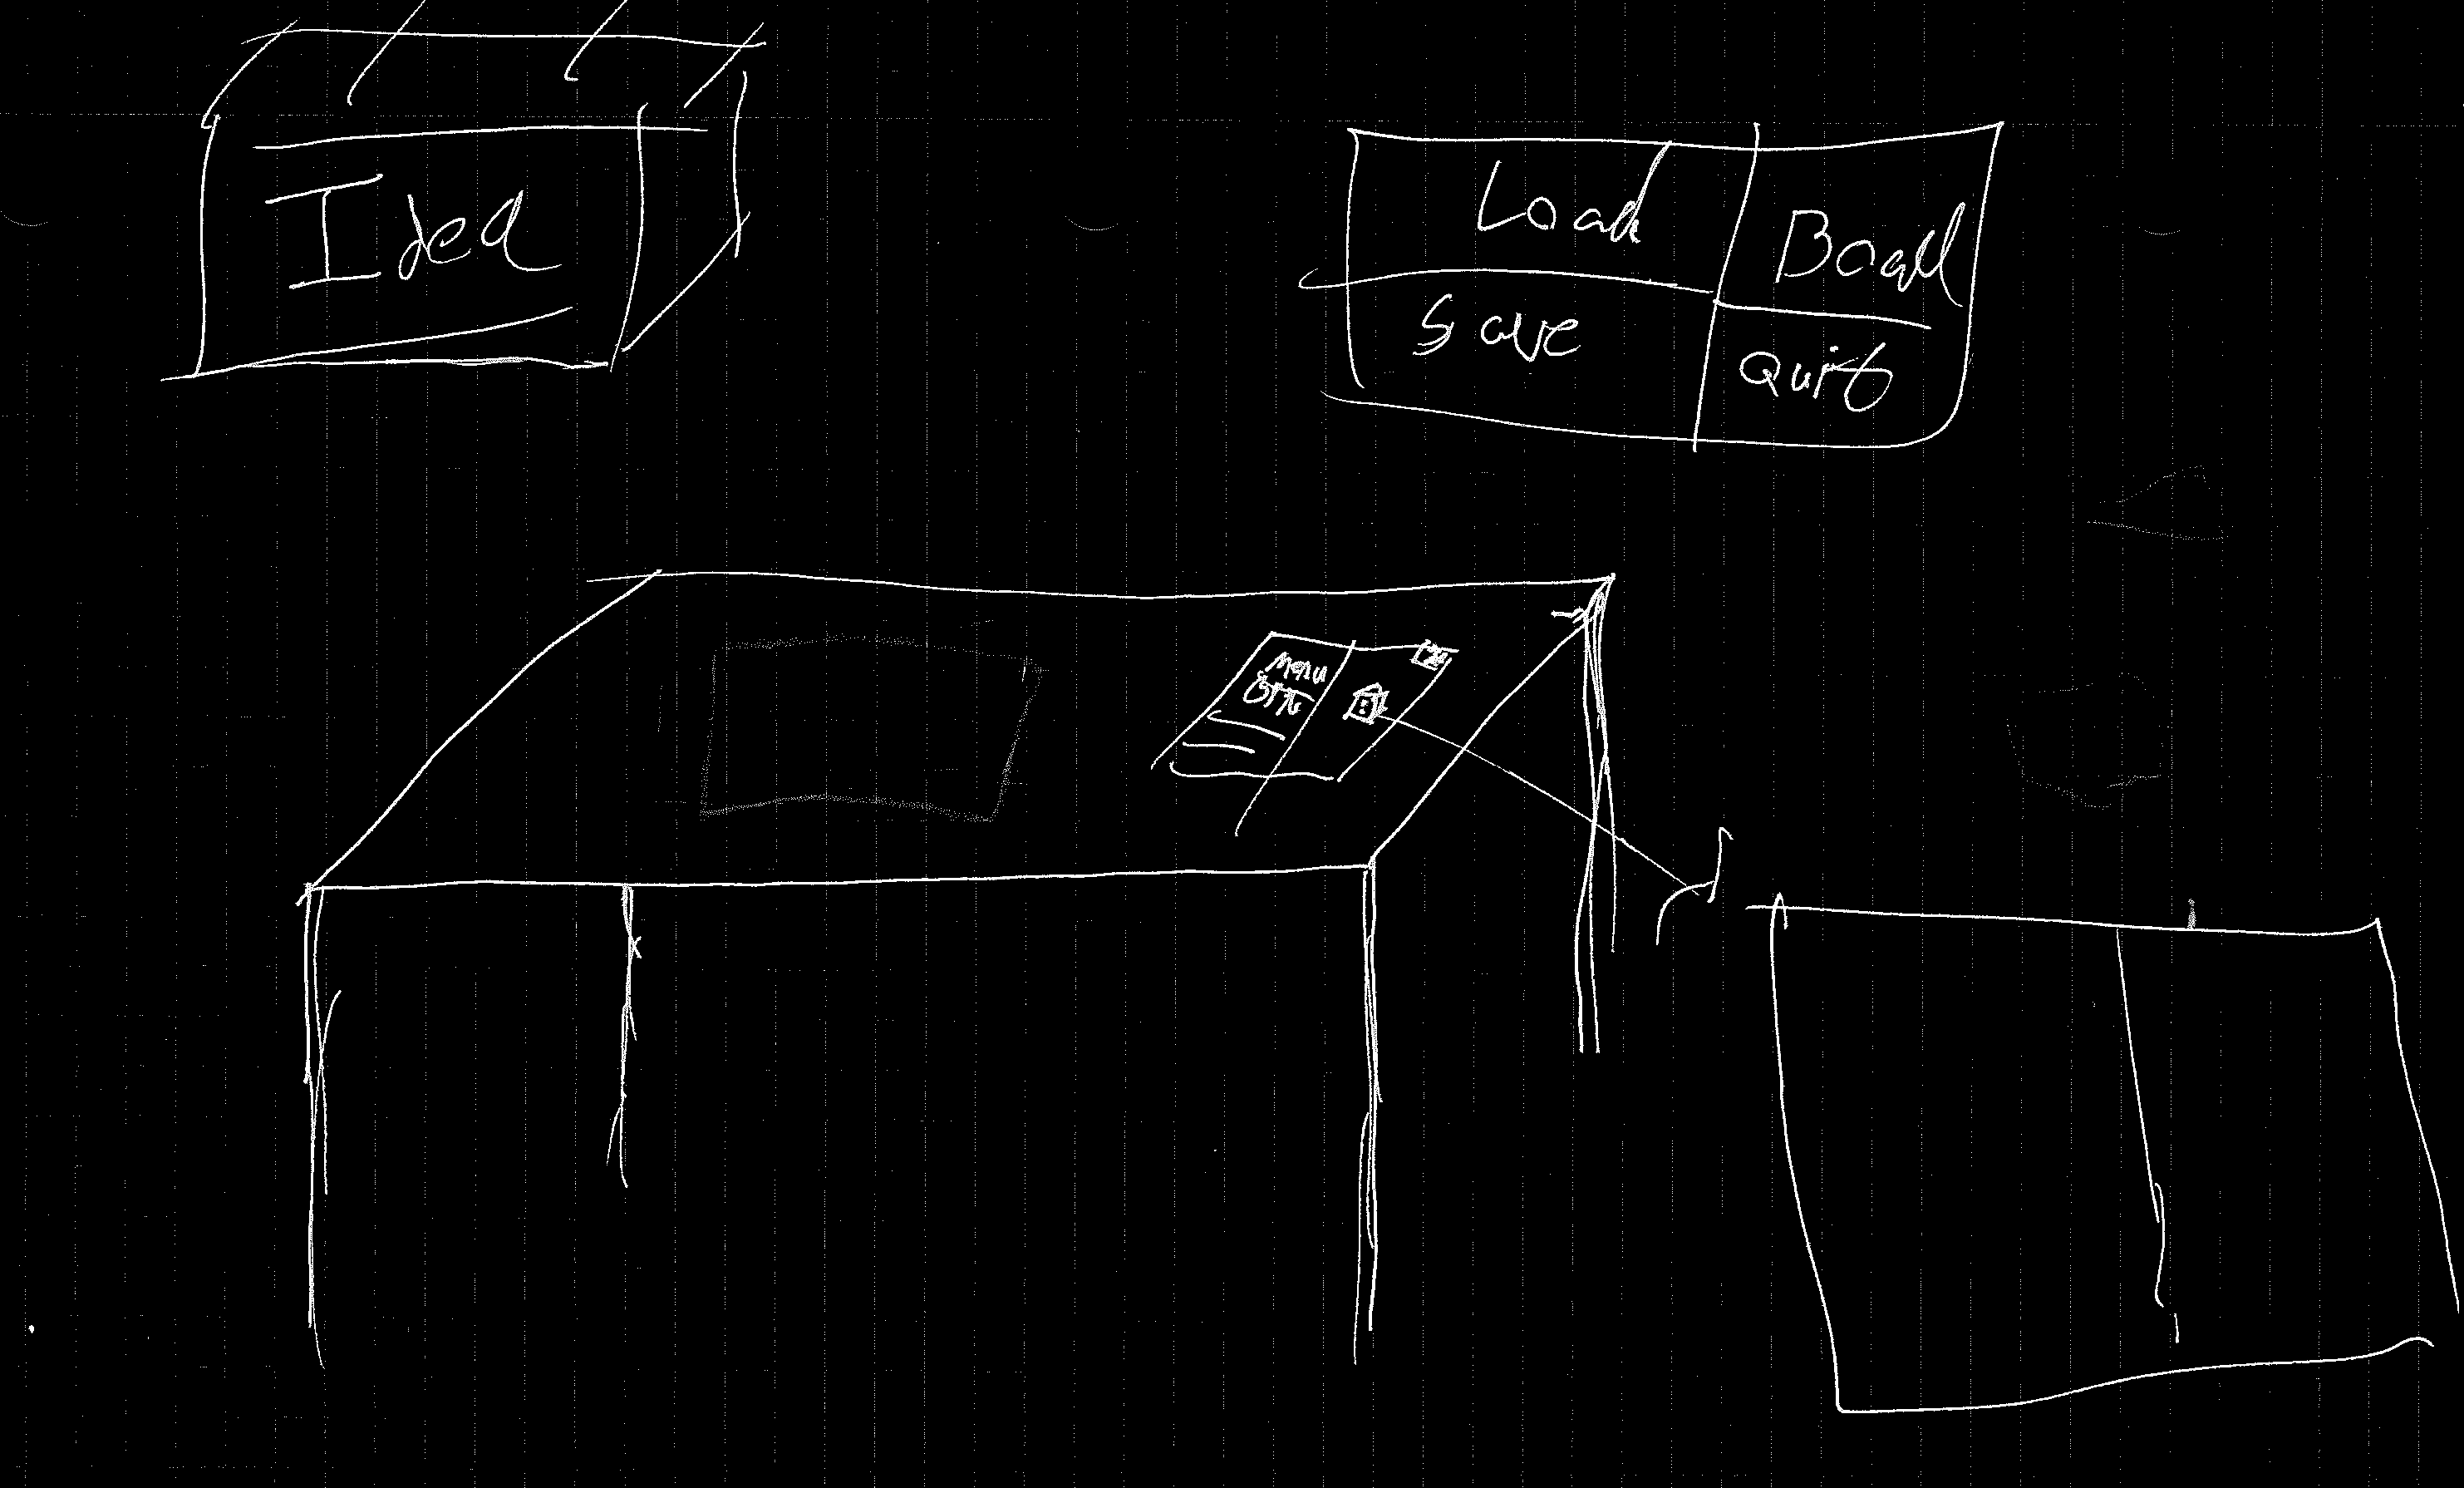
\includegraphics[width=210px]{figures/Generator/gen6.png}
	\caption{First sketch of the generator as a movable object. Here placed on the table, spawning blocks on the table.}~\label{fig:finaldesign}
\end{figure}
In the final design the user is met by a tablet device, consisting of large buttons with thumbnails and text explaining what each action does. As figure \ref{fig:finaldesign} shows, the user can choose different brick types and colors, as well as having a sandbox mode where a random amount of bricks are spawned to play with. The user can also spawn prebuilt templates, save/load previous sessions and go back to the main menu with a 'back' button. 

